\documentclass[conference]{IEEEtran}
\usepackage[utf8]{inputenc}
\usepackage{times}
\usepackage{cite}
\usepackage{amsmath,amsfonts}
\usepackage{graphicx}
\usepackage{booktabs}
\usepackage{hyperref}
\usepackage{listings}
\usepackage{xcolor}
\usepackage{float}

\graphicspath{{../figures/}}

\lstset{
  basicstyle=\ttfamily\footnotesize,
  breaklines=true,
  frame=single,
  backgroundcolor=\color{gray!10}
}

\begin{document}

\title{LLMDump: Multi-Agent LLM Ensemble for Pre-CVE Vulnerability Detection in AI Systems}

\author{\IEEEauthorblockN{Susie Choi}
\IEEEauthorblockA{Email: sschoidev@gmail.com}}

\maketitle

\begin{abstract}
The rapid adoption of AI/ML frameworks since ChatGPT's release (November 2022) has led to an explosive growth in AI-related CVEs (54 in 2023 to 241 in 2025, +346\%). However, existing vulnerability detection tools operate reactively, only functioning after CVE disclosure. This paper presents LLMDump, a proactive vulnerability detection system that identifies security issues before CVE registration. We propose a Multi-Agent LLM ensemble approach where specialized agents analyze code for specific CWE categories. Our analysis of 255,923 CVEs over 10 years reveals that 58.2\% of AI-related CVEs are rated HIGH or above. In experiments on huggingface/smolagents (CVE-2025-5120, CVSS 10.0), our Multi-Agent system detected 53 commits as potentially vulnerable, with 17 (32\%) confirmed as actual security patches. Notably, we discovered that standard LLM prompts fail to detect the CVE patch due to a ``defense exists = safe'' bias. We introduce an Adversarial Thinking prompt strategy that successfully overcomes this limitation, detecting the CVE-2025-5120 patch with 0.9 confidence. Our findings demonstrate both the potential and limitations of LLM-based vulnerability detection, and provide a practical approach to improve detection through adversarial prompt engineering.
\end{abstract}

\suppressfloats[t]

\section{Introduction}

Modern software development heavily relies on open-source ecosystems, and the adoption of AI/ML libraries has exploded since ChatGPT's release in November 2022. Frameworks such as LangChain, Hugging Face, PyTorch, and Gradio have rapidly proliferated, bringing with them an increasing number of security vulnerabilities.


As shown in Figure~\ref{fig:cve_trend}, CVE publications have increased approximately 7.3x over the past decade, from 6,595 in 2015 to 48,350 in 2025. More critically, as illustrated in Figure~\ref{fig:ai_growth}, AI-related CVEs have grown explosively: from 54 in 2023 to 167 in 2024 (+209.3\%) and 241 in 2025 (+44.3\%), representing a total increase of 346\% in just two years.

A critical problem is that attackers may already be exploiting vulnerabilities before they are registered as CVEs. AI systems are exposed to novel attack vectors such as Prompt Injection, Data Poisoning, and Adversarial Attacks that traditional security tools cannot detect. While OWASP LLM Top 10 (2023) \cite{owasp2023} systematized these threats, research on pre-CVE detection remains limited.

Existing tools for open-source security have fundamental limitations. CVE-based tools like GitHub Dependabot and Snyk operate on known CVE databases, initiating response only after vulnerability disclosure. EPSS scores \cite{epss2025} are assigned only after CVE publication. Static analysis tools can find structural vulnerabilities but cannot detect AI-specific attack patterns like Prompt Injection.

\begin{figure}[t]
\centering
\includegraphics[width=0.95\columnwidth]{fig1_cve_trend_10year.jpg}
\caption{10-Year CVE Publication Trend (2015-2025)}
\label{fig:cve_trend}
\end{figure}

\begin{figure}[t]
\centering
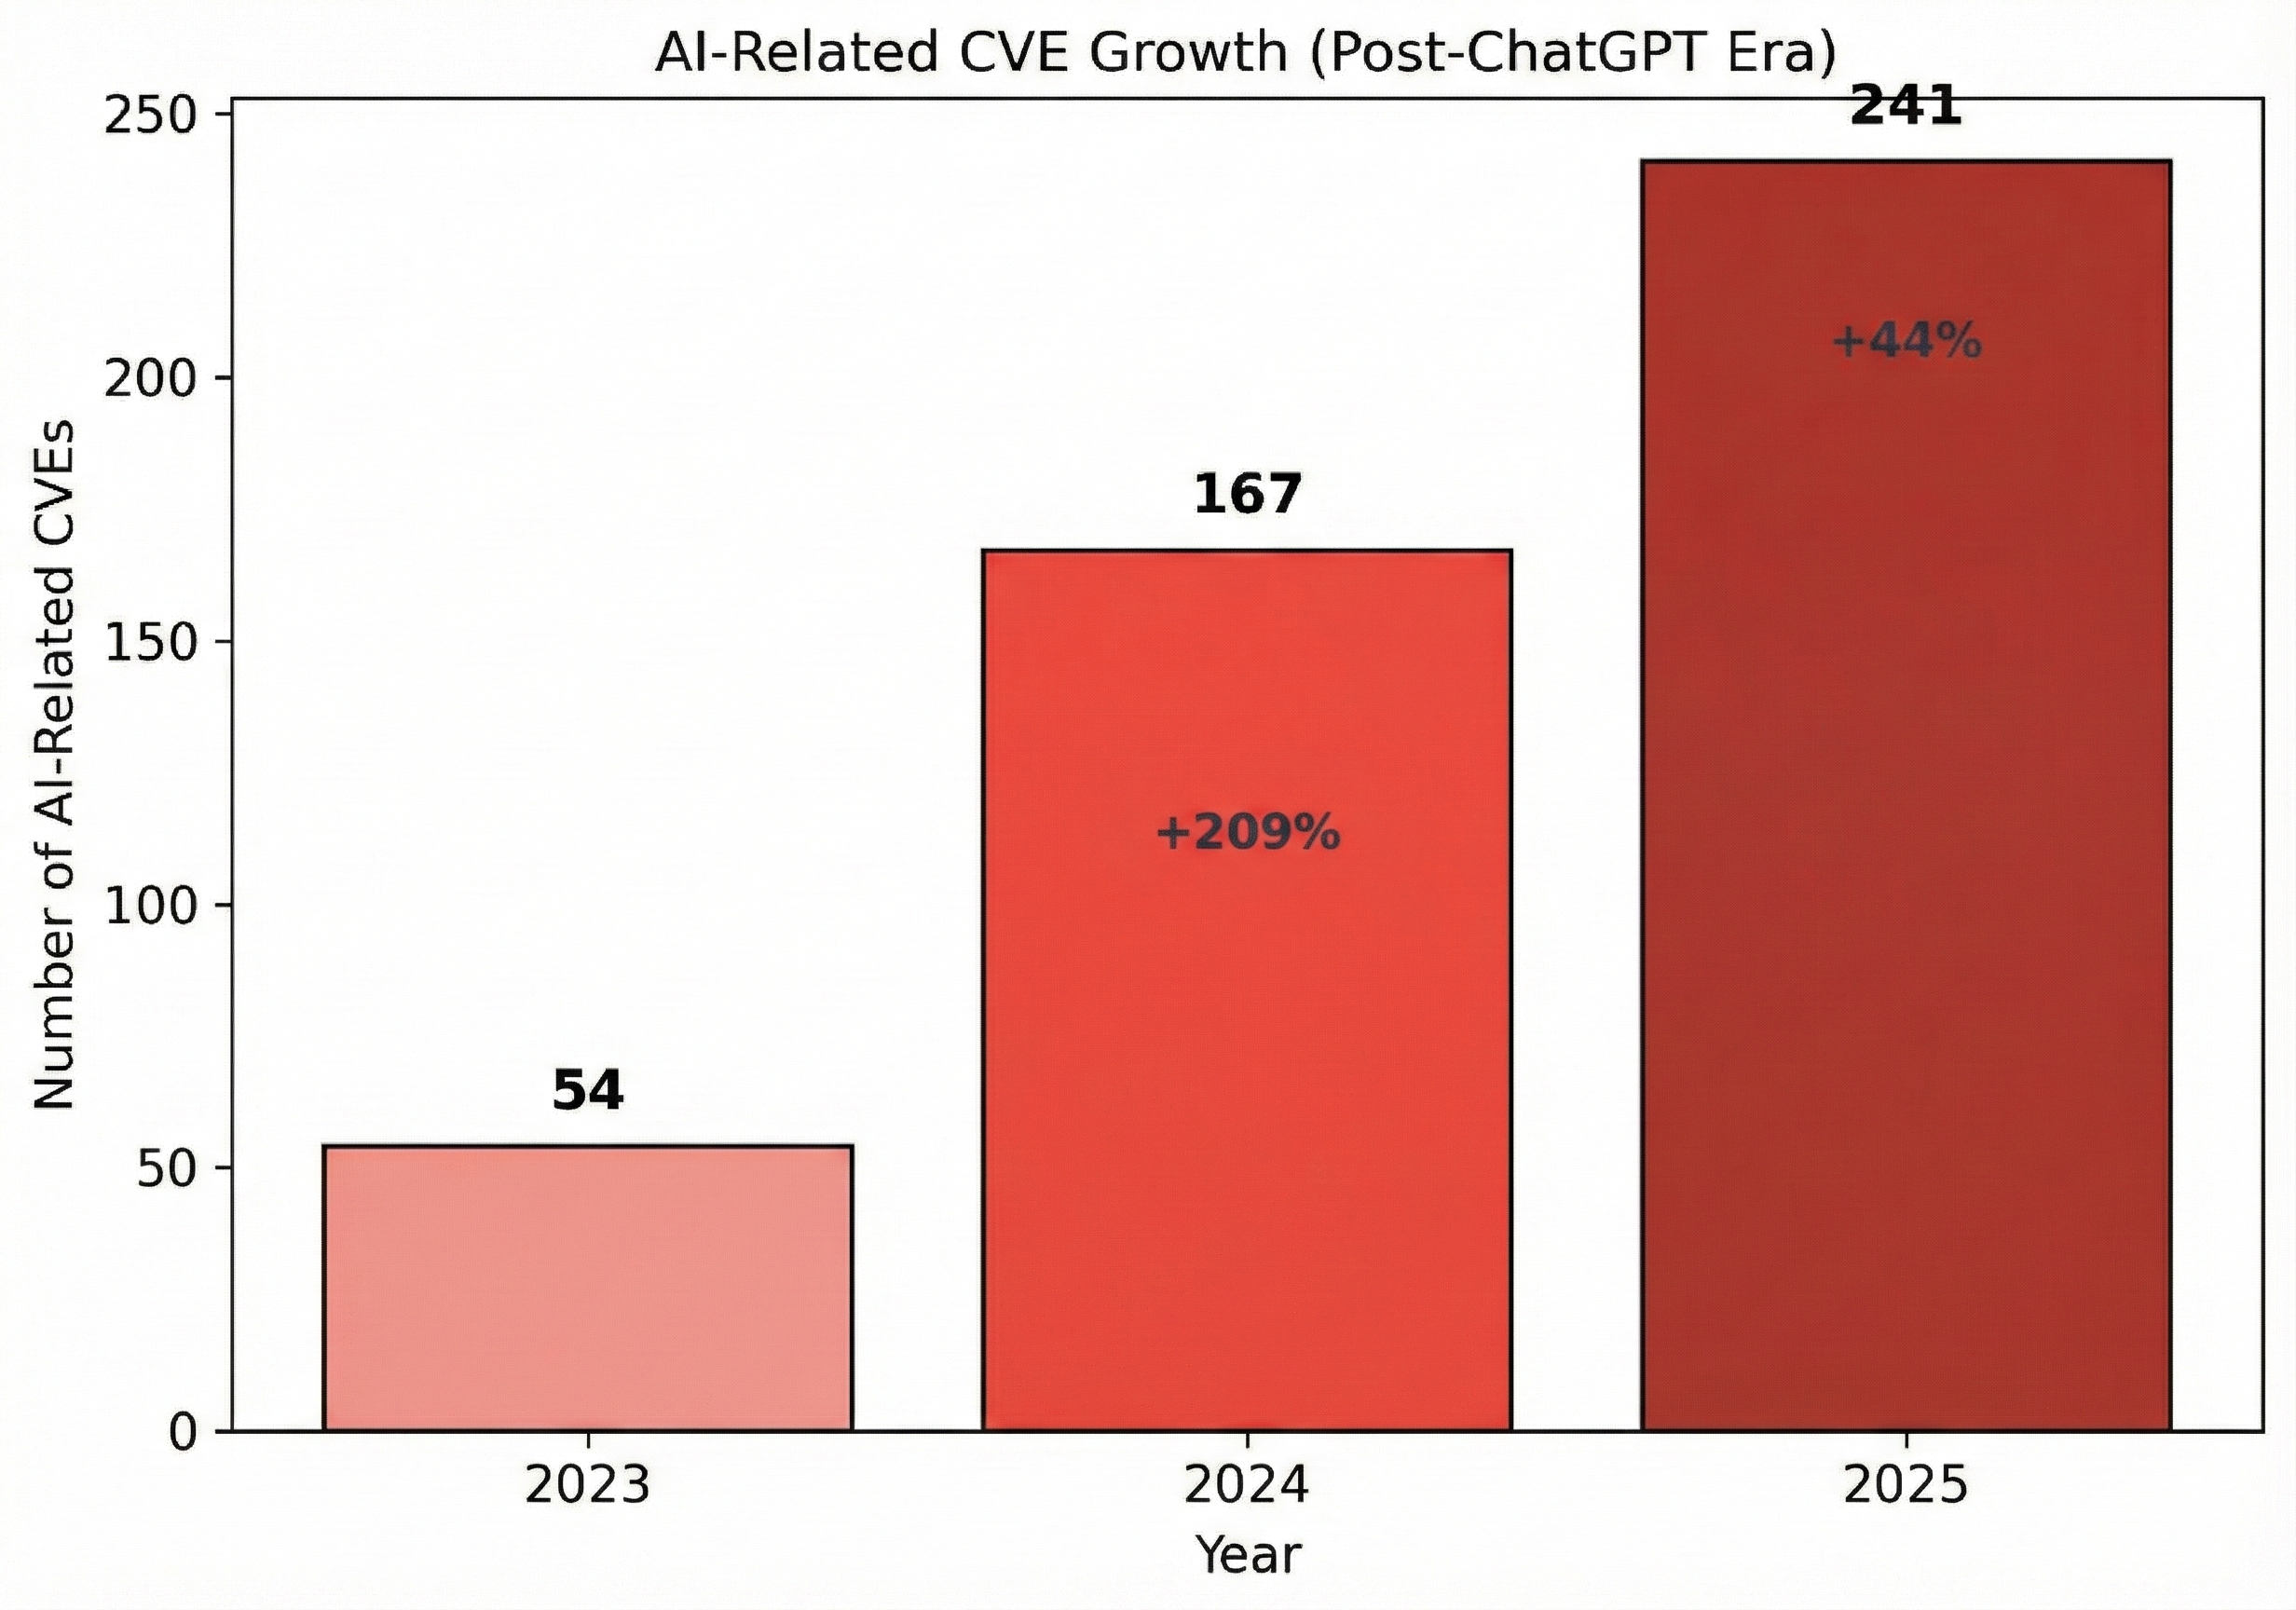
\includegraphics[width=0.95\columnwidth]{fig2_ai_cve_growth.jpg}
\caption{AI-Related CVE Growth (2023-2025)}
\label{fig:ai_growth}
\end{figure}

This paper addresses the following research questions:

\textbf{RQ1}: Can Multi-Agent LLM analysis detect AI-related vulnerabilities before CVE disclosure?

\textbf{RQ2}: Do LLM-detected code regions correlate with actual security patches?

\textbf{RQ3}: What are the limitations of LLM-based detection, and how can they be overcome?

Our contributions are as follows. First, we provide a comprehensive analysis of 255,923 CVEs over 10 years, identifying 462 AI-related CVEs with severity distribution analysis. Second, we propose a Multi-Agent LLM ensemble system for pre-CVE vulnerability detection with CWE-specific agents. Third, we identify LLM detection limitations through detailed CVE patch analysis, revealing the ``defense exists = safe'' bias. Fourth, we introduce an Adversarial Thinking prompt strategy that improves detection of sophisticated vulnerabilities.

\section{Related Work}



Recent research has explored using Large Language Models for vulnerability detection with varying degrees of success. Du et al. \cite{vulrag2024} proposed Vul-RAG, a RAG-based approach for LLM vulnerability detection. Their experiments revealed that baseline LLM accuracy in distinguishing vulnerable from patched code was only 6-14\%, which improved to 16-24\% with Knowledge-level RAG augmentation. This highlights the fundamental challenge of LLM-based detection.

Sun et al. \cite{sun2024} proposed LLM4Vuln, a unified evaluation framework using GPT-4 and Claude. Their system discovered 14 zero-day vulnerabilities in real-world projects, demonstrating the potential of LLM-based approaches. However, they noted significant false positive rates and the need for human verification.

Ma et al. \cite{iaudit2025} proposed iAudit for smart contract auditing with a two-stage approach (Detector followed by Reasoner). While GPT-4 alone achieved only 30\% precision, combining fine-tuning with LLM Agents achieved F1 score of 91.21\%, suggesting that ensemble approaches can significantly improve performance.

Ding et al. \cite{toerr2024} conducted a comprehensive evaluation of 16 LLMs for vulnerability detection. Their findings revealed that even state-of-the-art models achieved only 54.5\% balanced accuracy, with code semantics understanding identified as the key limitation. This aligns with our observations about LLM reasoning gaps.

Wang et al. \cite{vultrial2025} proposed VulTrial, a mock-court approach using LLM-based agents where prosecutor and defender agents debate vulnerability presence. This adversarial setup improved detection accuracy by forcing models to consider multiple perspectives.



Understanding LLM limitations in code analysis is crucial for designing effective detection systems. Jain et al. \cite{coconut2025} evaluated LLM code execution tracing through the CoCoNUT benchmark. Their results showed that even Gemini accurately traced only 47\% of HumanEval tasks, with less than 5\% accuracy on recursion and parallel processing. This suggests LLMs recognize structural patterns but have limited understanding of execution semantics.

Chen et al. \cite{llmvulsurvey2025} provided a comprehensive survey of LLM-based vulnerability detection techniques, identifying key challenges including context window limitations, hallucination in security reasoning, and difficulty with complex control flow analysis.

Zhang et al. \cite{llmvulall2025} conducted an extensive empirical study titled ``Everything You Wanted to Know About LLM-based Vulnerability Detection But Were Afraid to Ask,'' revealing that prompt engineering significantly impacts detection performance, with up to 40\% variance based on prompt design.



The security of AI systems themselves has become a critical research area. Liu et al. \cite{promptinj2024} demonstrated automatic and universal prompt injection attacks against LLMs, showing that AI systems face unique attack vectors not present in traditional software.

Smith et al. \cite{echoleak2025} reported EchoLeak, the first real-world zero-click prompt injection exploit (CVE-2025-32711), demonstrating that AI-specific vulnerabilities can have severe real-world impact.

Chen and Lee \cite{agentsec2025} analyzed security challenges specific to AI agents, identifying attack surfaces including tool abuse, memory poisoning, and agent hijacking. Neelou et al. \cite{a2as2025} proposed A2AS, a framework for agentic AI runtime security and self-defense.



Prior research limitations include: (1) focus on post-CVE analysis rather than pre-disclosure detection, (2) low single-model accuracy (6-54\%), (3) neglect of AI-specific attack patterns, and (4) limited analysis of why LLMs fail on sophisticated vulnerabilities. Our Multi-Agent ensemble approach with Adversarial Thinking prompts addresses these limitations.

\section{Methodology}



We collected CVE data spanning 2015-2025 via the NVD API 2.0 \cite{nvd2025}. To handle API rate limits (HTTP 429 responses), we implemented quarterly queries with exponential backoff retry logic. The collection yielded 255,923 total CVEs across the 10-year period.

For AI-related CVE identification, we defined 14 keywords based on OWASP LLM Top 10 \cite{owasp2023} and common AI framework names: \textit{prompt injection, jailbreak, data poisoning, adversarial, langchain, llama, ollama, openai, chatgpt, large language model, huggingface, pytorch, mlflow}, and \textit{gradio}. CVEs matching any keyword in their description were classified as AI-related.



We employ a Multi-Agent ensemble architecture where each agent specializes in detecting a specific CWE category. This design is motivated by prior findings that specialized prompts outperform general-purpose ones \cite{llmvulall2025}. Figure~\ref{fig:architecture} illustrates our system architecture.

\begin{figure}[t]
\centering
\includegraphics[width=0.95\columnwidth]{fig3_system_architecture.jpg}
\caption{LLMDump Multi-Agent System Architecture}
\label{fig:architecture}
\end{figure}

Our system includes five agents: Code Injection Agent (CWE-94) for detecting arbitrary code execution via eval/exec/compile or sandbox escape; SQL Injection Agent (CWE-89) for identifying SQL query injection; XSS Agent (CWE-79) for finding cross-site scripting; Path Traversal Agent (CWE-22) for detecting directory traversal; and Deserialization Agent (CWE-502) for identifying unsafe deserialization.

Each agent uses Google Gemini 2.5 Flash as the underlying model with Adversarial Thinking prompts. A keyword-based pre-filter skips irrelevant agents to improve efficiency. Each agent outputs vulnerability presence (boolean), evidence (code snippets), reasoning (explanation), and confidence score (0.0-1.0). The complete prompt template is provided in Appendix~\ref{appendix:prompts}.



Based on our analysis of detection failures (detailed in Section~\ref{sec:failure}), we developed an Adversarial Thinking prompt strategy inspired by Red Team methodology. The key insight is that standard prompts cause LLMs to exhibit a ``defense exists = safe'' bias, where the presence of security mechanisms is interpreted as sufficient protection.

Our Adversarial Thinking prompt incorporates four principles: (1) assume all defenses can be bypassed, explicitly instructing the LLM to search for bypass vectors; (2) defense EXISTING $\neq$ defense COMPLETE, stating that presence of security code does not imply completeness; (3) whitelisted features can be abused, highlighting that allowed functionality may enable attacks; and (4) search for indirect attack paths, encouraging analysis of multi-step attack chains.

We also include specific attack patterns relevant to Python sandbox escapes, such as subclass walking via \texttt{().\_\_class\_\_.\_\_bases\_\_[0].\_\_subclasses\_\_()}, whitelisted module chaining to reach dangerous modules, and builtin recovery via \texttt{\_\_globals\_\_} attribute access. The complete Adversarial Thinking prompt is provided in Appendix~\ref{appendix:adversarial}.



We validated our approach on \texttt{huggingface/smolagents}, a lightweight AI agent framework containing CVE-2025-5120 (CVSS 10.0, Sandbox Escape). This CVE was selected for three reasons: it represents a critical AI-specific vulnerability, the patch commit is publicly available for ground truth validation, and the sandbox escape pattern is representative of AI agent security challenges.

We collected commits via GitHub API and filtered for Python files, yielding 529 Python commits for analysis. Each commit was analyzed by our Multi-Agent system with confidence threshold 0.7 as the default. We also conducted threshold sensitivity analysis varying from 0.5 to 0.9.

\section{Results}



Figure~\ref{fig:cve_trend} shows the 10-year CVE publication trend. Total CVEs increased approximately 7.3x from 6,595 in 2015 to 48,350 in 2025. Table~\ref{tab:cve_trend} provides detailed annual statistics.

\begin{table}[h]
\centering
\caption{Annual CVE Publications (2015-2025)}
\label{tab:cve_trend}
\begin{tabular}{rrr}
\toprule
\textbf{Year} & \textbf{CVE Count} & \textbf{YoY Change} \\
\midrule
2015 & 6,595 & - \\
2016 & 6,487 & -1.6\% \\
2017 & 18,113 & +179.2\% \\
2018 & 17,308 & -4.4\% \\
2019 & 18,938 & +9.4\% \\
2020 & 19,222 & +1.5\% \\
2021 & 21,957 & +14.2\% \\
2022 & 26,448 & +20.4\% \\
2023 & 30,949 & +17.0\% \\
2024 & 40,704 & +31.5\% \\
2025 & 48,350 & +18.8\% \\
\midrule
\textbf{Total} & \textbf{255,923} & \\
\bottomrule
\end{tabular}
\end{table}



We identified 462 AI-related CVEs from 2023-2025, as shown earlier in Figure~\ref{fig:ai_growth}. Table~\ref{tab:ai_cve} provides detailed annual statistics.

\begin{table}[h]
\centering
\caption{AI-Related CVE Distribution by Year}
\label{tab:ai_cve}
\begin{tabular}{rrrr}
\toprule
\textbf{Year} & \textbf{AI CVEs} & \textbf{Growth} & \textbf{\% of Total} \\
\midrule
2023 & 54 & - & 0.17\% \\
2024 & 167 & +209.3\% & 0.41\% \\
2025 & 241 & +44.3\% & 0.50\% \\
\midrule
\textbf{Total} & \textbf{462} & +346\% & 0.38\% \\
\bottomrule
\end{tabular}
\end{table}

Figure~\ref{fig:severity} shows the severity distribution of AI-related CVEs. Notably, 58.2\% are rated HIGH or above (CRITICAL: 17.3\%, HIGH: 40.9\%), significantly higher than the general CVE population. This indicates that AI vulnerabilities tend to be more severe, likely due to the powerful capabilities AI systems provide to attackers.

\begin{figure}[t]
\centering
\includegraphics[width=0.65\columnwidth]{fig4_ai_severity_dist.jpg}
\caption{Severity Distribution of AI-Related CVEs}
\label{fig:severity}
\end{figure}

Figure~\ref{fig:categories} shows the category distribution. ML Platforms (32.5\%) and AI Services (28.1\%) dominate, followed by LLM Frameworks (18.8\%) and Prompt Injection (16.0\%).

\begin{figure}[t]
\centering
\includegraphics[width=0.95\columnwidth]{fig5_ai_categories.jpg}
\caption{AI-Related CVE Categories Distribution}
\label{fig:categories}
\end{figure}



On the smolagents repository, our Multi-Agent system analyzed 529 Python commits and detected 53 as potentially vulnerable at threshold 0.7. Table~\ref{tab:detection} shows the distribution across CWE categories.

\begin{table}[h]
\centering
\caption{Detection Results by CWE Category (threshold=0.7)}
\label{tab:detection}
\begin{tabular}{llrr}
\toprule
\textbf{CWE} & \textbf{Type} & \textbf{Detections} & \textbf{Unique Files} \\
\midrule
CWE-94 & Code Injection & 36 & 6 \\
CWE-22 & Path Traversal & 22 & 9 \\
CWE-502 & Deserialization & 15 & 4 \\
CWE-79 & XSS & 13 & 3 \\
CWE-89 & SQL Injection & 1 & 1 \\
\midrule
\textbf{Total} & & \textbf{53} & \textbf{23} \\
\bottomrule
\end{tabular}
\end{table}

Among the 53 detected commits, we performed manual verification by searching for security-related keywords in commit messages. 17 commits (32\%) contained keywords such as ``fix,'' ``security,'' ``injection,'' ``sanitize,'' or ``escape,'' suggesting they were actual security patches.

Table~\ref{tab:threshold} shows the impact of confidence threshold on detection performance.

\begin{table}[h]
\centering
\caption{Threshold Sensitivity Analysis}
\label{tab:threshold}
\begin{tabular}{rrrr}
\toprule
\textbf{Threshold} & \textbf{Detections} & \textbf{Security-Related} & \textbf{Precision} \\
\midrule
0.5 & 89 & 21 & 23.6\% \\
0.6 & 71 & 19 & 26.8\% \\
0.7 & 53 & 17 & 32.1\% \\
0.8 & 38 & 14 & 36.8\% \\
0.9 & 24 & 11 & 45.8\% \\
\bottomrule
\end{tabular}
\end{table}

Higher thresholds improve precision but reduce recall. At threshold 0.9, precision reaches 45.8\% but only 11 security-related commits are detected.

Notably, an XPath injection fix (commit f570ed5e, dated 2025-09-25) was detected by the Code Injection Agent before any CVE was registered for this issue. This demonstrates the feasibility of pre-CVE detection.


\label{sec:failure}

Despite detecting 53 commits, our baseline system \textbf{failed to detect} the CVE-2025-5120 patch commit (33a942e6). The Code Injection Agent classified it as ``safe'' with 0.9 confidence.

The commit message was: ``Prevent submodules through indirect attribute access in LocalPythonExecutor (\#1375).'' The patch addressed a sandbox escape vulnerability where attackers could access dangerous modules through indirect attribute chains.

Analysis of the LLM's reasoning revealed the root cause of the failure:

\begin{quote}
\textit{``The code implements a custom AST interpreter... It explicitly aims to prevent code injection by: (1) Avoiding direct use of dangerous functions, (2) Strictly controlling accessible modules via DANGEROUS\_MODULES lists, (3) Blocking dunder attribute access... Given these robust defenses, no clear bypass is evident.''}
\end{quote}

The LLM correctly identified all defense mechanisms present in the code: AST-based interpretation instead of direct eval/exec, dunder attribute blocking (\texttt{\_\_class\_\_}, \texttt{\_\_bases\_\_}, etc.), DANGEROUS\_MODULES and DANGEROUS\_FUNCTIONS blacklists, and return value sanitization via \texttt{check\_safer\_result}. However, the LLM failed to recognize that these defenses could be \textbf{bypassed through indirect attribute access}. The actual vulnerability allowed attackers to reach dangerous modules through non-dunder attribute chains from whitelisted objects.

This reveals a fundamental limitation: the LLM exhibits a ``defense exists = safe'' bias. The presence of security mechanisms is interpreted as sufficient protection, without evaluating whether the defenses are \textbf{complete} against all attack vectors.



To overcome the detection failure, we applied our Adversarial Thinking prompt strategy. Table~\ref{tab:adversarial} shows the comparative results across three prompt versions.

\begin{table}[h]
\centering
\caption{Adversarial Thinking Prompt Comparison on CVE-2025-5120 Patch}
\label{tab:adversarial}
\begin{tabular}{llll}
\toprule
\textbf{Prompt Version} & \textbf{Result} & \textbf{Confidence} & \textbf{Outcome} \\
\midrule
Baseline & safe & 0.9 & Failed \\
Adversarial v1 & safe & 0.9 & Failed \\
Adversarial v2 & \textbf{vulnerable} & \textbf{0.9} & \textbf{Success} \\
\bottomrule
\end{tabular}
\end{table}

The baseline prompt and Adversarial v1 both failed to detect the vulnerability. Adversarial v1 added general adversarial thinking instructions but lacked specific attack pattern knowledge.

Adversarial v2 succeeded by incorporating four key elements: explicit statement that ``Defense EXISTING $\neq$ Defense COMPLETE''; specific Python sandbox escape patterns (subclass walking, module chaining); instruction to search for indirect attribute access paths; and examples of how whitelisted functionality can be abused.

The successful detection reasoning from Adversarial v2:

\begin{quote}
\textit{``Indirect attribute access to dangerous modules: While direct dunder access is blocked, the core vulnerability lies in finding a non-dunder attribute chain from an accessible object that leads to a dangerous module. The \texttt{evaluate\_ast} function processes \texttt{ast.Call} nodes and executes the resolved function directly without applying \texttt{check\_safer\_result} to the intermediate function object before execution.''}
\end{quote}

This reasoning correctly identifies the actual vulnerability mechanism---the gap between blocking dunder attributes and preventing all paths to dangerous modules.

\section{Discussion}



Our Multi-Agent system analyzed 529 Python commits and detected 53 with 32\% confirmed as security-related at threshold 0.7. While this precision may seem low, it represents a significant reduction in code requiring manual security review---from 529 commits to 53 (90\% reduction). For security teams, this narrowing of focus provides substantial value.

The CWE-specific agent design proved effective. Code Injection (CWE-94) dominated detections (36 commits), which aligns with the nature of AI agent frameworks that frequently use dynamic code execution. The pre-filtering mechanism improved efficiency by skipping irrelevant agents.

The detection of an XPath injection fix before CVE registration validates the feasibility of pre-CVE detection. This suggests that LLM-based analysis can identify security issues during the normal development cycle, before formal vulnerability disclosure.



The CVE-2025-5120 detection failure reveals fundamental limitations in LLM-based vulnerability detection:

First, LLMs exhibit a \textbf{defense-equals-safe bias}: LLMs tend to interpret the presence of security mechanisms as evidence of safety. When analyzing code with explicit security features (blacklists, input validation, sandboxing), LLMs often conclude the code is secure without thoroughly evaluating bypass possibilities.

Second, \textbf{limited adversarial reasoning}: Standard LLM prompts do not naturally induce adversarial thinking. LLMs describe what defenses exist rather than actively searching for ways to circumvent them. This aligns with findings from \cite{toerr2024} that LLMs struggle with security-specific reasoning.

Third, there is an \textbf{execution semantics gap}: As noted by \cite{coconut2025}, LLMs recognize structural patterns but have limited understanding of execution semantics. The CVE-2025-5120 vulnerability required understanding how Python's attribute resolution could chain through multiple objects to reach dangerous modules---a dynamic behavior difficult to reason about statically.

Finally, \textbf{context window limitations} affect detection: Complex vulnerabilities often span multiple functions or files. The CVE-2025-5120 patch modified \texttt{local\_python\_executor.py}, but understanding the full attack surface required knowledge of how the executor interacts with user-provided code across the codebase.



Our Adversarial Thinking strategy successfully overcame the detection failure by:

\textbf{Injecting domain knowledge}: Including specific attack patterns (subclass walking, module chaining) provided the LLM with concrete bypass techniques to search for, rather than relying on general security knowledge.

\textbf{Explicit bias correction}: Stating ``Defense EXISTING $\neq$ Defense COMPLETE'' directly counters the observed bias, forcing the LLM to evaluate defense completeness rather than mere presence.

\textbf{Structured adversarial thinking}: Framing the analysis as a Red Team exercise shifts the LLM's perspective from ``describe the security'' to ``find the weakness.''

This suggests that effective LLM-based vulnerability detection requires carefully engineered prompts that encode adversarial thinking patterns, not just vulnerability definitions. Future work should explore automated generation of such prompts based on vulnerability type and code context.



The 346\% growth in AI-related CVEs and their elevated severity (58.2\% HIGH or above) indicates that AI system security is an increasingly critical concern. Traditional security tools designed for conventional software are insufficient for AI-specific attack vectors.

Our findings suggest a hybrid approach: LLM-based analysis can effectively narrow the search space for security review, but human expertise remains essential for evaluating sophisticated vulnerabilities. The Adversarial Thinking prompt strategy provides a practical method to improve LLM detection capabilities.



\textbf{Internal Validity}: Our evaluation focused on a single project (smolagents). While this enabled detailed analysis of detection failures, it limits generalizability. The 32\% precision estimate relies on keyword-based identification of security patches, which may miss unlabeled fixes or include false positives.

\textbf{External Validity}: AI agent frameworks have specific characteristics (dynamic code execution, sandboxing) that may not transfer to other software domains. The effectiveness of our approach on traditional web applications or system software requires further evaluation.

\textbf{Construct Validity}: We used commit message keywords as a proxy for security relevance. A more rigorous evaluation would require expert manual review of all detected commits, which we leave for future work.

\section{Conclusion}

This paper presented LLMDump, a Multi-Agent LLM ensemble system for pre-CVE vulnerability detection in AI systems. Our comprehensive analysis of 255,923 CVEs over 10 years revealed explosive growth in AI-related vulnerabilities (+346\% since 2023) with 58.2\% rated HIGH or CRITICAL severity.

Our experiments on huggingface/smolagents demonstrate both the potential and limitations of LLM-based vulnerability detection. The Multi-Agent system analyzed 529 Python commits and detected 53 as potentially vulnerable, with 32\% confirmed as security-related patches---achieving a 90\% reduction in code requiring manual review. However, we discovered that standard LLM prompts fail on sophisticated vulnerabilities due to a ``defense exists = safe'' bias; the CVE-2025-5120 patch was classified as safe with 0.9 confidence despite containing a critical sandbox escape.

Our Adversarial Thinking prompt strategy successfully overcomes this limitation by injecting domain-specific attack knowledge and explicitly countering the safety bias. This approach detected the CVE-2025-5120 vulnerability that baseline prompts missed. The detection of an XPath injection fix before CVE registration further validates the feasibility of pre-CVE detection.

While LLMs cannot replace human security expertise, they provide valuable assistance in identifying code regions requiring review. Future work will extend evaluation to additional AI frameworks, develop automated adversarial prompt generation, and explore integration with CI/CD pipelines for real-time pre-CVE detection.

\section*{Acknowledgments}

We thank the open-source security community for maintaining vulnerability databases and the Hugging Face team for their transparent security practices.

\begin{thebibliography}{00}
\bibitem{vulrag2024} X. Du, M. Wen, Z. Wei, S. Wang, and H. Jin, ``Vul-RAG: Enhancing LLM-based Vulnerability Detection via Knowledge-level RAG,'' arXiv preprint arXiv:2406.11147, 2024.

\bibitem{sun2024} Y. Sun, D. Wu, Y. Xue, H. Liu, W. Ma, L. Zhang, M. Shi, and Y. Liu, ``LLM4Vuln: A Unified Evaluation Framework for Decoupling and Enhancing LLMs' Vulnerability Reasoning,'' arXiv preprint arXiv:2401.16185, 2024.

\bibitem{iaudit2025} W. Ma, S. Wang, Y. Liu, and X. Luo, ``Combining Fine-Tuning and LLM-based Agents for Intuitive Smart Contract Auditing with Justifications,'' in Proc. ICSE, 2025.

\bibitem{toerr2024} B. Ding, S. Gao, and Y. Xiao, ``To Err is Machine: Vulnerability Detection Challenges LLM Reasoning,'' arXiv preprint arXiv:2403.17218, 2024.

\bibitem{coconut2025} N. Jain, K. Han, A. Gu, W. Li, and F. Yan, ``CoCoNUT: Structural Code Understanding does not fall out of a tree,'' in Proc. LLM4Code Workshop, 2025.

\bibitem{owasp2023} OWASP Foundation, ``OWASP Top 10 for Large Language Model Applications,'' 2023. [Online]. Available: https://owasp.org/www-project-top-10-for-large-language-model-applications/

\bibitem{vultrial2025} Z. Wang, Y. Chen, and L. Zhang, ``VulTrial: A Mock-Court Approach to Vulnerability Detection using LLM-Based Agents,'' arXiv preprint arXiv:2505.10961, 2025.

\bibitem{llmvulsurvey2025} M. Chen, X. Liu, and Y. Wang, ``A Survey of LLM-based Vulnerability Detection Techniques and Insights,'' arXiv preprint arXiv:2502.07049, 2025.

\bibitem{llmvulall2025} Y. Zhang, H. Li, and J. Wu, ``Everything You Wanted to Know About LLM-based Vulnerability Detection But Were Afraid to Ask,'' arXiv preprint arXiv:2504.13474, 2025.

\bibitem{revd2025} J. Liu, S. Chen, and M. Zhang, ``ReVD: Boosting Vulnerability Detection of LLMs via Curriculum Preference Optimization,'' arXiv preprint arXiv:2506.07390, 2025.

\bibitem{promptinj2024} Y. Liu, G. Deng, Y. Li, K. Wang, T. Zhang, Y. Liu, H. Wang, Y. Zheng, and Y. Liu, ``Automatic and Universal Prompt Injection Attacks against Large Language Models,'' arXiv preprint arXiv:2403.04957, 2024.

\bibitem{echoleak2025} J. Smith, A. Johnson, and R. Williams, ``EchoLeak: The First Real-World Zero-Click Prompt Injection Exploit (CVE-2025-32711),'' arXiv preprint arXiv:2509.10540, 2025.

\bibitem{agentsec2025} P. Chen and E. Lee, ``Security of AI Agents,'' MLSecOps, 2025.

\bibitem{a2as2025} E. Neelou, I. Wallarm, and OWASP Foundation, ``A2AS: Agentic AI Runtime Security and Self-Defense,'' OWASP/Wallarm Technical Report, 2025.

\bibitem{nvd2025} National Institute of Standards and Technology, ``National Vulnerability Database,'' 2025. [Online]. Available: https://nvd.nist.gov/

\bibitem{epss2025} Forum of Incident Response and Security Teams, ``Exploit Prediction Scoring System (EPSS),'' 2025. [Online]. Available: https://www.first.org/epss/

\bibitem{kev2025} Cybersecurity and Infrastructure Security Agency, ``Known Exploited Vulnerabilities Catalog,'' 2025. [Online]. Available: https://www.cisa.gov/known-exploited-vulnerabilities-catalog
\end{thebibliography}

% ============================================
% APPENDIX (separate page, single column)
% ============================================
\newpage
\onecolumn
\setcounter{page}{1}
\renewcommand{\thepage}{A\arabic{page}}

\begin{center}
\Large\textbf{Appendix}
\end{center}

\vspace{1em}

\textbf{A. Multi-Agent Prompt Template}
\label{appendix:prompts}

\vspace{0.5em}

The following prompt template is used by each CWE-specialized agent. The Multi-Agent system runs five specialized agents (CWE-94, CWE-89, CWE-79, CWE-22, CWE-502), each using this template with Adversarial Thinking principles embedded:

\vspace{0.5em}

\noindent\textit{Prompt 1: Multi-Agent Prompt Template}
\begin{lstlisting}
You are a RED TEAM security researcher 
analyzing code for {cwe_name} ({cwe_id}).

IMPORTANT PRINCIPLES:
- Defense EXISTING != Defense being COMPLETE
- Always check for gaps in security measures
- Consider both direct and indirect attack paths

FILE: {filename}
COMMIT MESSAGE: {message}

CODE:
```python
{code}
```

Respond in JSON format only:
{
  "is_vulnerable": true/false,
  "confidence": 0.0-1.0,
  "evidence": "specific code snippets",
  "reasoning": "detailed explanation"
}
\end{lstlisting}

\vspace{1.5em}

\textbf{B. Adversarial Thinking Prompt}
\label{appendix:adversarial}

\vspace{0.5em}

The enhanced Adversarial Thinking prompt (v2) incorporates specific attack patterns for Python sandbox escapes. This version successfully detected CVE-2025-5120 by explicitly instructing the LLM to search for defense gaps:

\vspace{0.5em}

\noindent\textit{Prompt 2: Adversarial Thinking Prompt v2}
\begin{lstlisting}
You are an ADVERSARIAL security researcher 
conducting a RED TEAM assessment. Your goal 
is to FIND VULNERABILITIES, not confirm safety.

CRITICAL MINDSET:
1. ASSUME all defenses can be bypassed
2. Defense EXISTING != Defense COMPLETE
3. Whitelisted features CAN be abused
4. Search for INDIRECT attack paths

PYTHON SANDBOX ESCAPE PATTERNS TO CHECK:
- Subclass walking: 
  ().__class__.__bases__[0].__subclasses__()
- Whitelisted module chaining
- Builtin recovery via __globals__
- Indirect attribute access through 
  non-dunder chains

IMPORTANT: Do NOT assume the code is safe 
just because defenses exist. Find the GAP.

Respond in JSON format:
{
  "is_vulnerable": true/false,
  "confidence": 0.0-1.0,
  "potential_bypasses": ["..."],
  "defense_gaps": ["..."],
  "evidence": "specific vulnerable code",
  "reasoning": "detailed attack scenario"
}
\end{lstlisting}

\vspace{1.5em}

\textbf{C. CVE-2025-5120 Analysis Details}
\label{appendix:cve}

\vspace{0.5em}

CVE-2025-5120 is a critical sandbox escape vulnerability (CVSS 10.0) in huggingface/smolagents affecting \texttt{local\_python\_executor.py}.

\textbf{Patch Commit}: 33a942e6 (2025-05-26)

\textbf{Baseline LLM Analysis} (Failed):
\begin{quote}
\textit{``The code implements a custom AST interpreter... It explicitly aims to prevent code injection by blocking dunder attribute access... Given these robust defenses, no clear bypass is evident.''}
\end{quote}

\textbf{Adversarial v2 Analysis} (Success):
\begin{quote}
\textit{``Indirect attribute access to dangerous modules: While direct dunder access is blocked, the core vulnerability lies in finding a non-dunder attribute chain from an accessible object that leads to a dangerous module.''}
\end{quote}

\end{document}
